
%\documentclass[12pt]{article}
\documentclass[conference]{IEEEtran}

\usepackage{graphicx}
\graphicspath{ {assets/} }

\usepackage{xcolor}
\usepackage[margin=1in]{geometry}
\usepackage{setspace}
\usepackage{amsmath}
\usepackage{amssymb}
\usepackage{booktabs}
\usepackage{graphicx}
\usepackage{float}
\usepackage{tikz}
\usetikzlibrary{arrows.meta,positioning}
\usepackage{pifont}
\usepackage{hyperref}

% Stage colours used in the process-flow TikZ figure
\colorlet{cpwt}{blue!70!black}
\colorlet{cwao}{green!55!black}
\colorlet{cet}{violet!80!black}
\colorlet{cat}{blue!80!black}
% Command to mark a section as completed
\newcommand{\completedsection}[1]{{\color{green!60!black}\section{#1}}}

\title{Research Plan: COD Prediction in Wastewater Treatment}
\author{Ong Jai Sheng}
\date{\today}

\begin{document}
\maketitle
\onehalfspacing

Core Question: How do different temporal feature engineering strategies (Raw Sensor Baseline vs.\ Kalman Filtering vs.\ Kalman+ARIMA) and different modelling architectures (Traditional Machine Learning vs.\ Deep Learning) affect out-of-sample $R^2$ performance when predicting wastewater \texttt{AT\_COD}?


\section{Introduction}


\section{Materials and Methods}

\subsection{Dataset and Biological Treatment Process}

To maintain industrial confidentiality, the dataset used in this study was derived by applying a controlled stochastic perturbation to operational measurements from an active biological wastewater treatment facility. Specifically, independent Gaussian noise with a standard deviation of 0.5\% of each variable's observed range was applied to the original sensor readings, producing a statistically representative simulated dataset that preserves the temporal dynamics and inter-variable relationships of the real process while preventing proprietary data disclosure. The resulting dataset comprised 983 chronological daily observations spanning the full operational record of the facility.

The treatment process follows a four-stage pipeline, illustrated in Fig.~\ref{fig:process_flow}. Raw industrial wastewater first enters the Process Wastewater Tank (PWT), which acts as a primary collection and homogenisation buffer. The wastewater then passes through Wet Air Oxidation (WAO), a thermochemical pre-treatment stage that breaks down refractory organic compounds prior to biological treatment. The partially oxidised effluent subsequently enters the Equalization Tank (ET), which stabilises flow and load variability before the final biological stage. The aeration tank (AT) constitutes the core activated sludge reactor, where aerobic microorganisms mineralise residual organic matter under controlled aeration.

\begin{figure}[H]
\centering
\resizebox{\linewidth}{!}{%
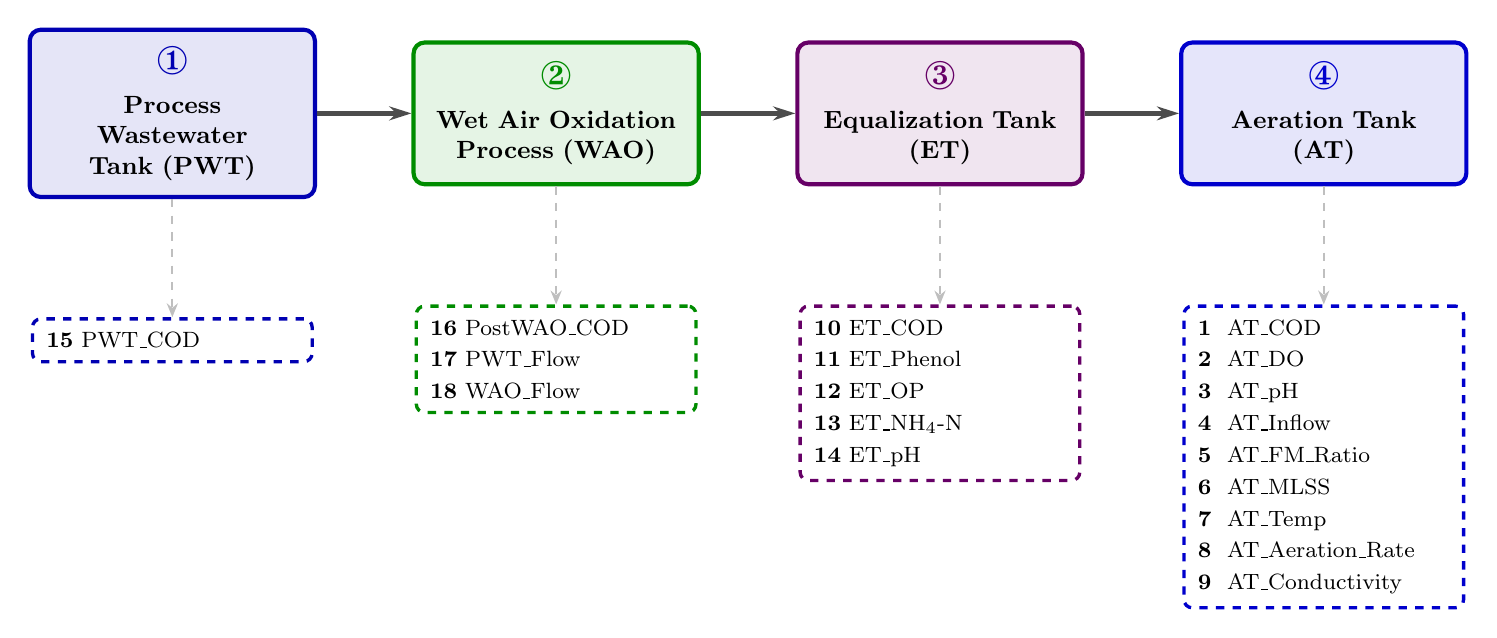
\begin{tikzpicture}[
    font=\small,
    box/.style={rounded corners=4pt, line width=1.5pt,
                text width=3.2cm, align=center,
                inner sep=6pt, minimum height=1.8cm},
    varbox/.style={dashed, rounded corners=3pt, line width=1.2pt,
                   text width=3.2cm, align=left, inner sep=5pt,
                   font=\footnotesize},
    mainarrow/.style={-{Stealth[length=8pt,width=5pt]},
                      line width=2pt, draw=gray!60!black},
    dasharrow/.style={-{Stealth[length=5pt,width=4pt]},
                      dashed, thick, draw=gray!50},
]

%% ---- Stage header boxes ----------------------------------------
\node[box, draw=cpwt, fill=cpwt!10] (s1)
    {\textcolor{cpwt}{\Large\ding{172}}\\[3pt]
     \textbf{Process Wastewater}\\
     \textbf{Tank (PWT)}};

\node[box, draw=cwao, fill=cwao!10, right=1.2cm of s1] (s2)
    {\textcolor{cwao}{\Large\ding{173}}\\[3pt]
     \textbf{Wet Air Oxidation}\\
     \textbf{Process (WAO)}};

\node[box, draw=cet, fill=cet!10, right=1.2cm of s2] (s3)
    {\textcolor{cet}{\Large\ding{174}}\\[3pt]
     \textbf{Equalization Tank}\\
     \textbf{(ET)}};

\node[box, draw=cat, fill=cat!10, right=1.2cm of s3] (s4)
    {\textcolor{cat}{\Large\ding{175}}\\[3pt]
     \textbf{Aeration Tank}\\
     \textbf{(AT)}};

%% ---- Process flow arrows ---------------------------------------
\draw[mainarrow] (s1.east) -- (s2.west);
\draw[mainarrow] (s2.east) -- (s3.west);
\draw[mainarrow] (s3.east) -- (s4.west);

%% ---- Variable boxes --------------------------------------------
\node[varbox, draw=cpwt, below=1.5cm of s1] (v1)
    {\textbf{15}~PWT\_COD};

\node[varbox, draw=cwao, below=1.5cm of s2] (v2)
    {\textbf{16}~PostWAO\_COD\\[2pt]
     \textbf{17}~PWT\_Flow\\[2pt]
     \textbf{18}~WAO\_Flow};

\node[varbox, draw=cet, below=1.5cm of s3] (v3)
    {\textbf{10}~ET\_COD\\[2pt]
     \textbf{11}~ET\_Phenol\\[2pt]
     \textbf{12}~ET\_OP\\[2pt]
     \textbf{13}~ET\_NH$_4$-N\\[2pt]
     \textbf{14}~ET\_pH};

\node[varbox, draw=cat, below=1.5cm of s4] (v4)
    {\textbf{1}~~AT\_COD\\[2pt]
     \textbf{2}~~AT\_DO\\[2pt]
     \textbf{3}~~AT\_pH\\[2pt]
     \textbf{4}~~AT\_Inflow\\[2pt]
     \textbf{5}~~AT\_FM\_Ratio\\[2pt]
     \textbf{6}~~AT\_MLSS\\[2pt]
     \textbf{7}~~AT\_Temp\\[2pt]
     \textbf{8}~~AT\_Aeration\_Rate\\[2pt]
     \textbf{9}~~AT\_Conductivity};

%% ---- Dashed drop arrows ----------------------------------------
\draw[dasharrow] (s1.south) -- (v1.north);
\draw[dasharrow] (s2.south) -- (v2.north);
\draw[dasharrow] (s3.south) -- (v3.north);
\draw[dasharrow] (s4.south) -- (v4.north);

\end{tikzpicture}%
}
\caption{Four-stage industrial wastewater treatment pipeline.
         Solid arrows denote the direction of wastewater flow.
         Dashed arrows indicate the sensor variables collected at
         each stage; \texttt{AT\_COD}~(1) and \texttt{AT\_DO}~(2)
         are the primary prediction targets, and all remaining
         variables serve as input features.}
\label{fig:process_flow}
\end{figure}

The two primary prediction targets in this study are the Chemical Oxygen Demand within the aeration tank (AT\_COD), which quantifies the residual organic load at the biological treatment stage, and the Dissolved Oxygen concentration (AT\_DO), which governs aerobic microbial activity and process efficiency. The remaining variables across all four process stages serve as input features. Table~\ref{tab:variables} summarises the full set of measured variables, their abbreviations, and their roles in the predictive modelling pipeline.

\begin{table}[H]
    \caption{Measured Process Variables Grouped by Treatment Stage}
    \label{tab:variables}
    \centering
    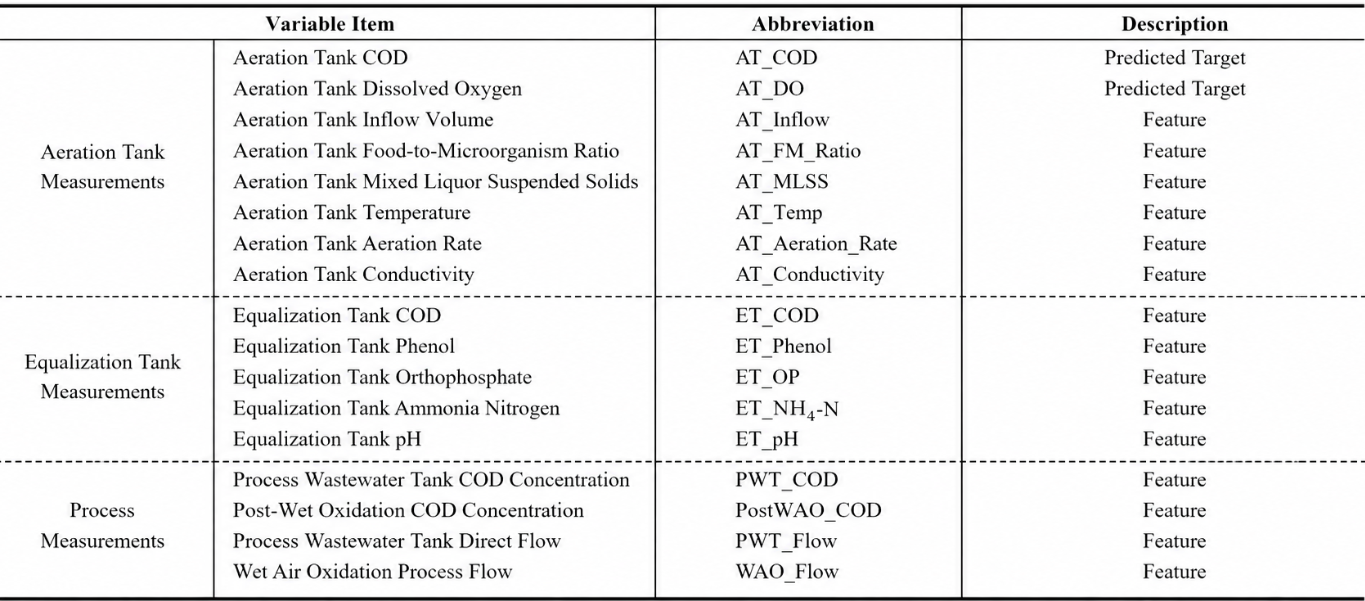
\includegraphics[width=\linewidth]{dataset.png}
\end{table}

A fundamental physical constraint governing this process is the aeration tank's hydraulic retention time of approximately six days. Consequently, influent quality fluctuations required up to six days to manifest in the effluent, meaning contemporaneous sensor readings did not reflect instantaneous cause-and-effect relationships. This temporal delay dictated the time-series architecture of the predictive models: input features were constructed as six-day rolling averages of the process variables to forecast the aeration tank state six days ahead, strictly aligning the machine learning formulation with the physical dynamics of the system.

\subsection{Target-Derived Feature Engineering (The Kalman/ARIMA Pipeline)}
% [To be filled]

\subsection{Proposed Regression Architecture: Extra Trees}

% [To be filled]

\subsection{Deep Learning Benchmark (Phase 3 LSTM Optimization)}

% [To be filled]

\subsection{Experimental Setup and Evaluation Metrics}

% [To be filled]

\section{Results and Discussion}


\section{Conclusion}

\section{References}

Takuya Akiba, Shotaro Sano, Toshihiko Yanase, Takeru Ohta, and Masanori Koyama. 2019.
	Optuna: A Next-generation Hyperparameter Optimization Framework. In KDD.


%\begin{itemize}
%    \item \textbf{The Story:} Feature engineering (like writing Kalman filter code) takes a lot of human effort. What if we used an AI that naturally understands time all by itself (raw data fed directly into an LSTM neural network)?
%    \item \textbf{The Evidence:} You introduce \textbf{LSTM (Deep Learning)}. Because LSTM has literal ``memory cells'' built into its code, you test whether it can beat your meticulously engineered PLS model.
%    \item \textbf{The Grand Finale:} You present the final comparison. Did human math (Kalman + PLS) beat the deep learning method (LSTM), which is the ultimate "Rolling Modeling Approach."
%\end{itemize}
\end{document}
